\documentclass[master.tex]{subfiles}

\begin{document}
\setlength{\intextsep}{5pt} \setlength{\columnsep}{10pt}

\section*{D. Research Design and Methods}

\subsection*{Aim 1: Study the temporal window of prospective and retrospective
  memory linking.}

% \begin{figure}[!hbt]
%   \centering 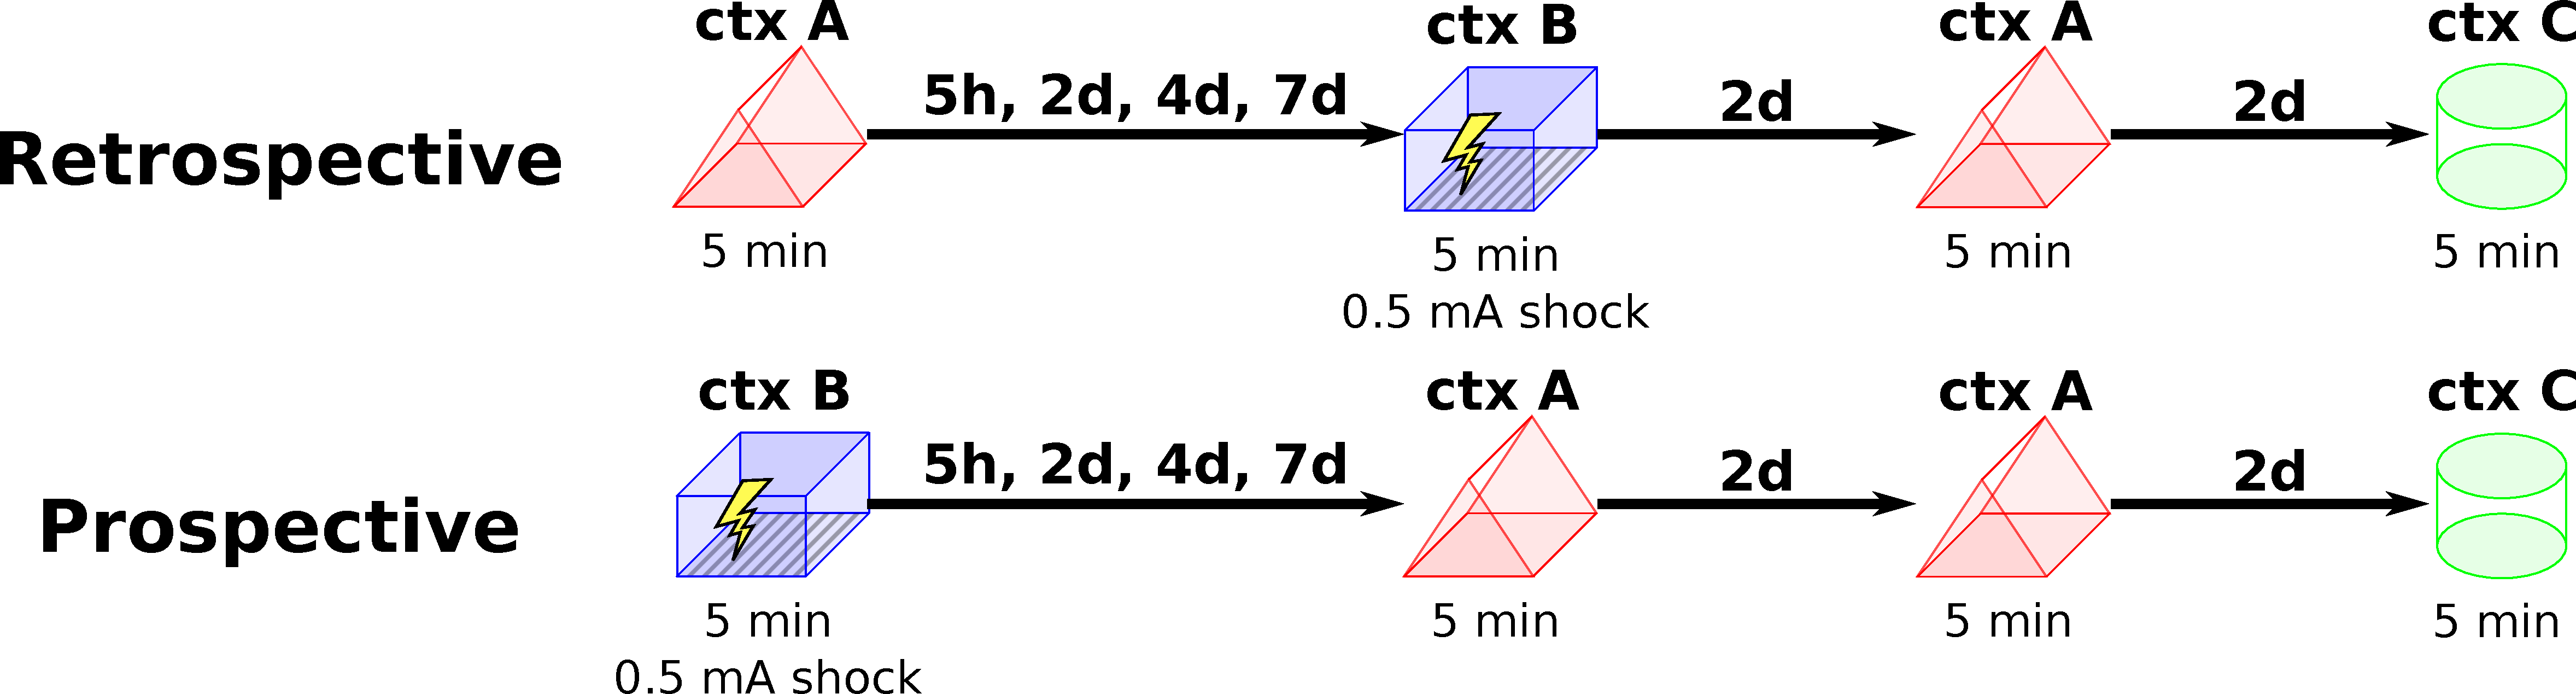
\includegraphics[scale = .135]{Figures/exp_pro_retro.pdf}
%   \caption{\footnotesize behavior experimental design.}
%   \label{fig:exp_behav}
% \end{figure}

\begin{wrapfigure}{L}{0.6\textwidth}
  \centering 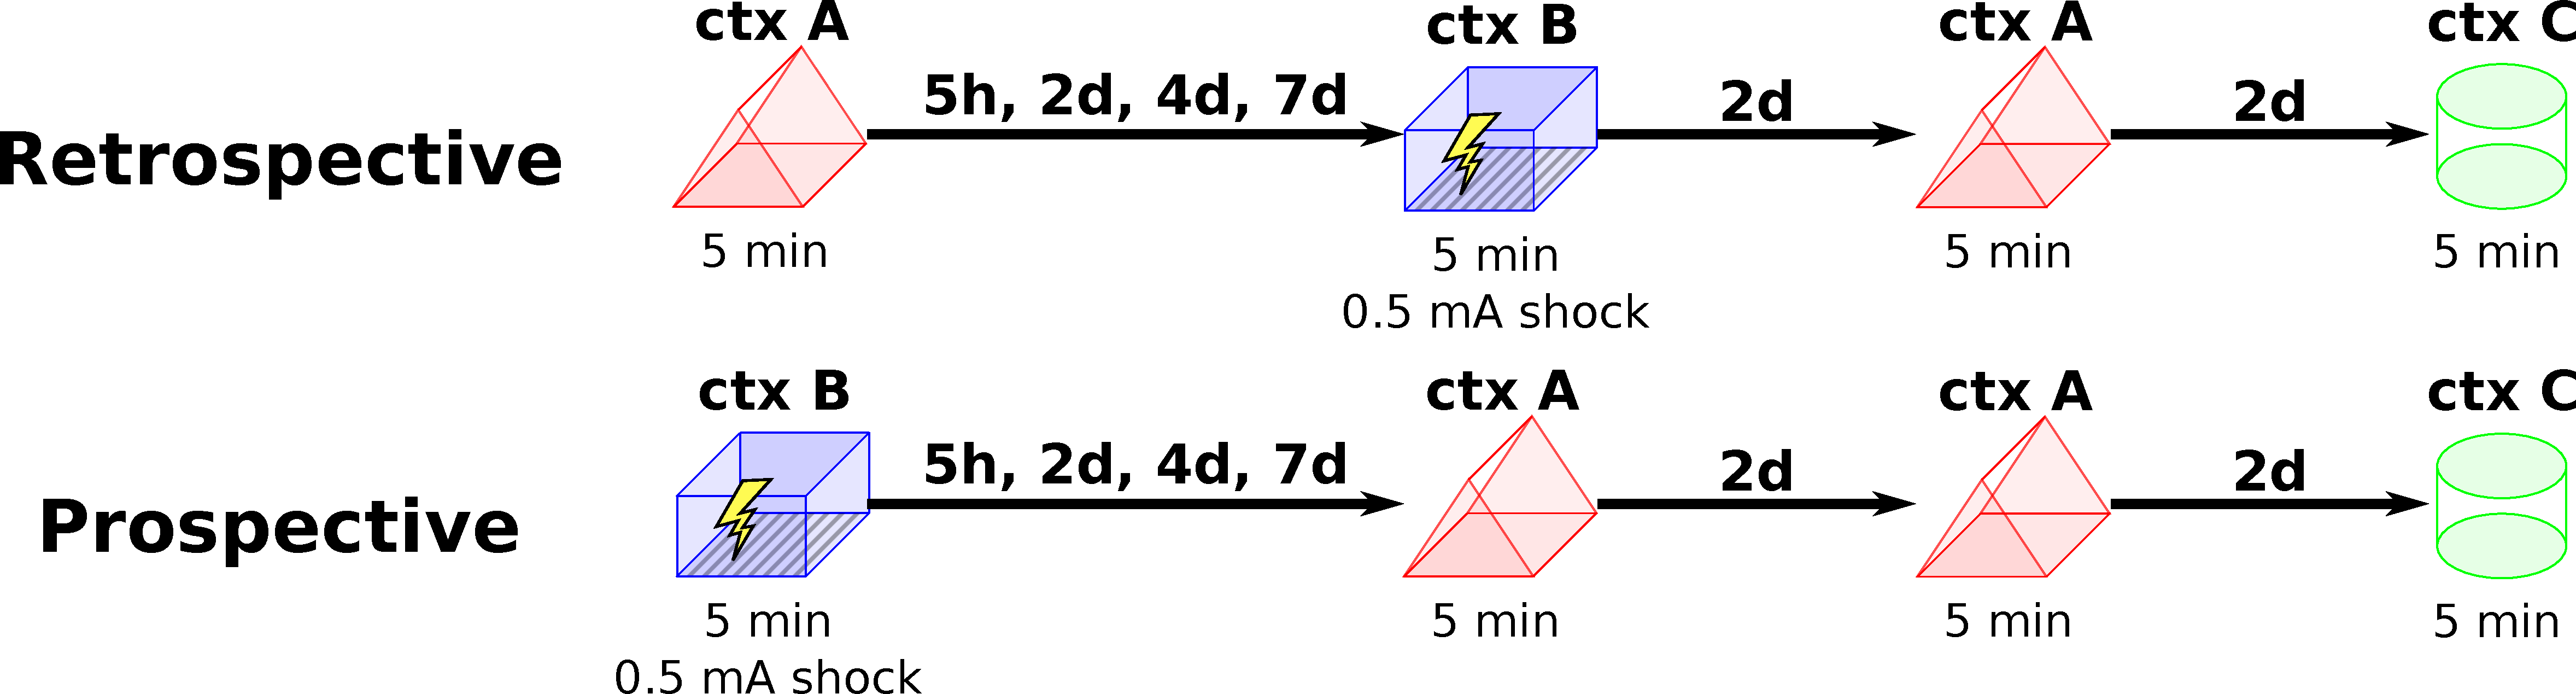
\includegraphics[width=0.6\textwidth]{Figures/exp_pro_retro.pdf}
  \caption{\footnotesize behavior experimental design.}
  \label{fig:exp_behav}
\end{wrapfigure}

To test hypothesis that retrospective memory linking has a longer temporal
window than prospective memory linking, we will carry out behavior studies as
shown in \autoref{fig:exp_behav}. Specifically, animals will be put into two
distinct contexts and separated into two major groups where the temporal order
of the two contexts during encoding is opposite. In the ``prospective'' group,
animals will receive a delayed shock in context B first, and then explore
context A, whereas in ``retrospective'' group, animals will explore context A
first, and then get a delayed shock in context B. For both groups, the
exploration sessions will last for 5 minutes, and a foot shock of 0.5 mA will be
delivered at second minute during the encoding session of context B. After
encoding, both groups will be tested in context A and a novel context C in that
order 2 days after they are exposed to both context A and B. The time interval
between the two testing session will be 2 days. During testing, animals'
behavior will be recorded, and freezing level will be assessed from the videos
using standard software (Med Associates, Inc.). Within each major group, the
animals will be further divided into subgroups, and will be equally assigned to
either 5 hours, 1 day, 2 days or 7 days subgroup, which indicates the time
interval between the exposure of context A and B. Then, within each subgroup,
animals' freezing level in context A during testing can be compared with those
in the novel context C. An elevated freezing level in context A, where no shock
ever occurred for all groups, relative to the novel context C, indicates a
transfer of fear from context B to context A. Then within each major group, we
can estimate the temporal window of memory linking by looking at whether context
A and B are linked together with each temporal intervals. Finally, the temporal
window for retrospective and prospective memory linking can be compared between
the two major groups. We expect to see retrospective memory linking across 2
days, while the temporal window of prospective memory linking will be shorter
than 1 day.

The presented experimental design has 8 unique groups in total. We plan to have
12 animals assigned to each group, resulting in a total of 96 animals for the
presented study. The experiment is expected to be finished within 6 months.

One concern of the presented experimental design is the order effect of testing
sequence, where testing in one of the context will affect freezing level in the
other context that is tested later. To control for this, we will switch the
testing order of context A and context C in selected groups. If order effect are
observed, we can adopt an alternative ``parallel'' testing design, where animals
within each group can be further divided into two groups, with half of the
animals being tested in context A only, and the other half being tested in
context C only.

\subsection*{Aim 2: Study how ensemble dynamic contribute to memory linking.}

% \begin{figure}[!hbt]
%   \centering 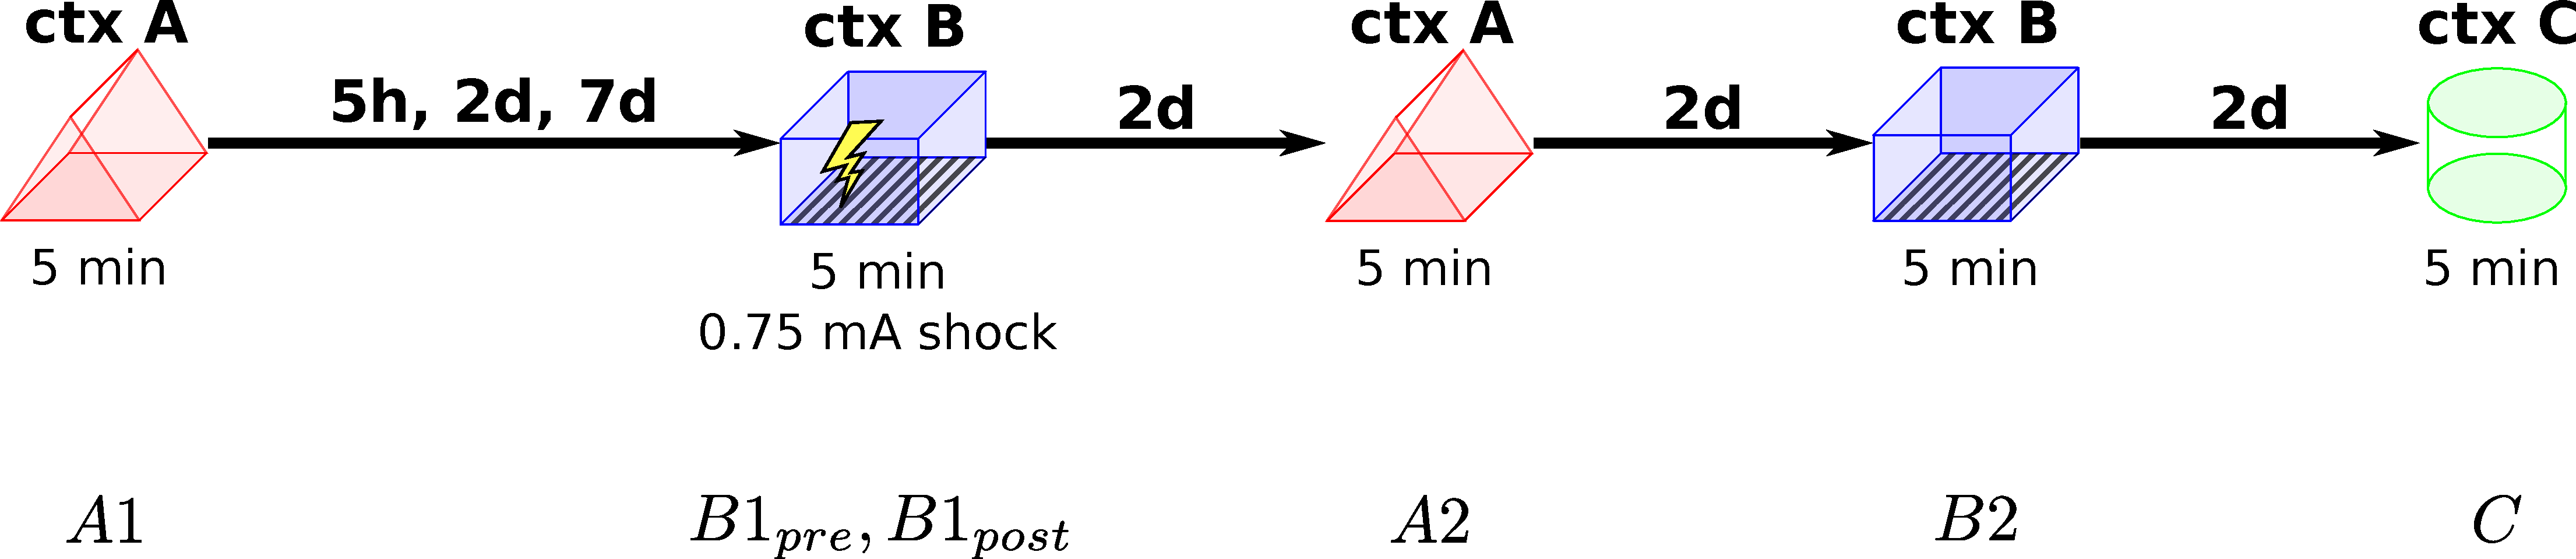
\includegraphics[scale = .135]{Figures/exp_imag.pdf}
%   \caption{\footnotesize imaging experiment design.}
%   \label{fig:exp_imag}
% \end{figure}

\begin{wrapfigure}{L}{0.6\textwidth}
  \centering 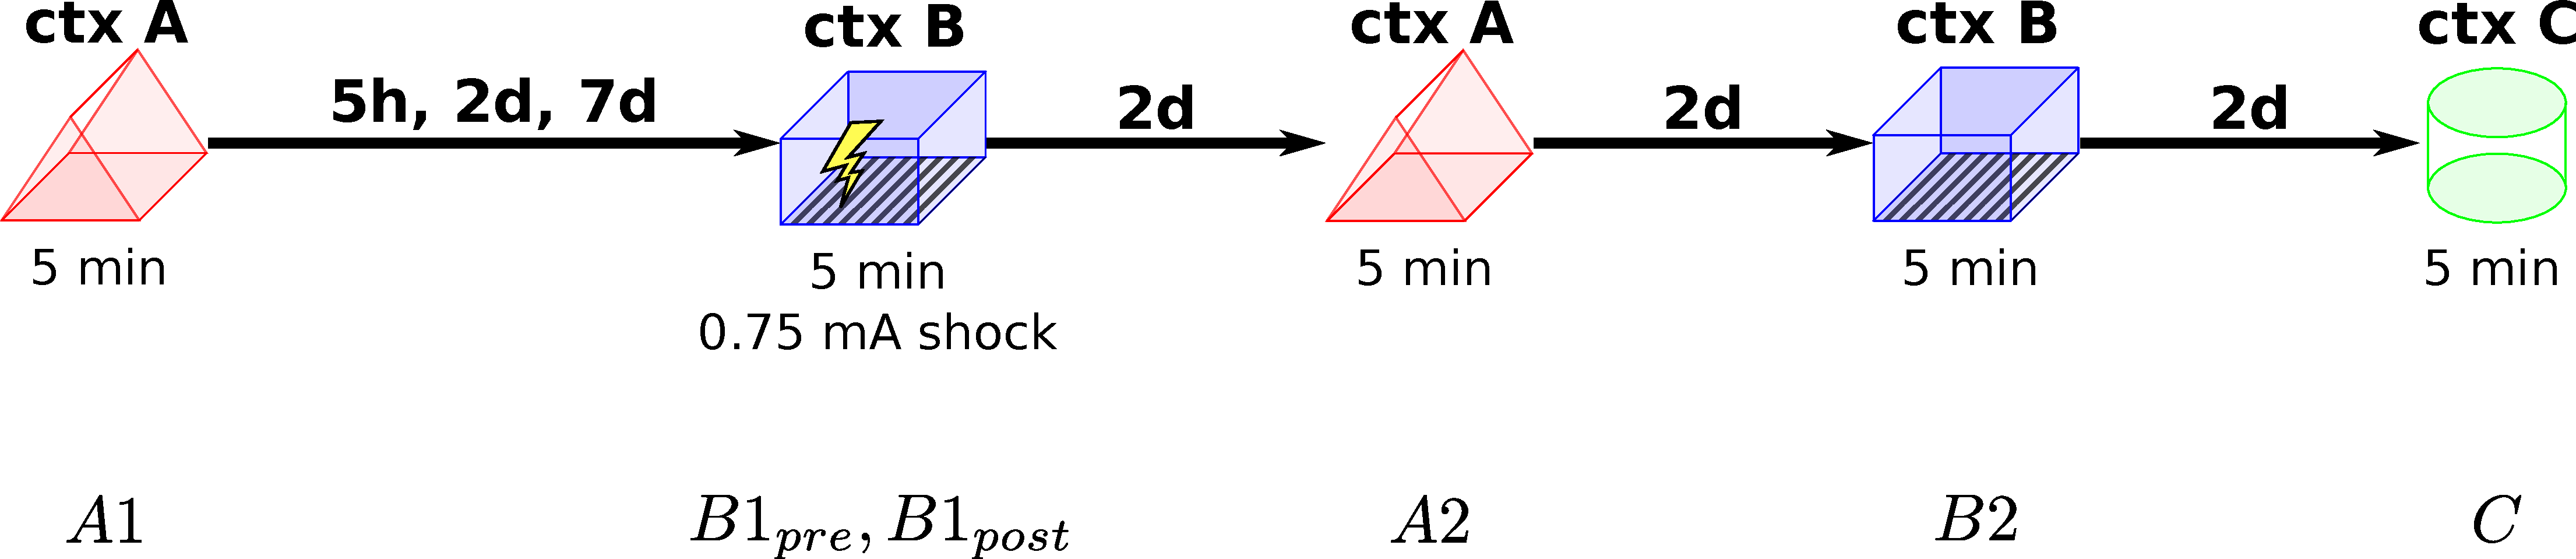
\includegraphics[width=0.6\textwidth]{Figures/exp_imag.pdf}
  \caption{\footnotesize imaging experiment design.}
  \label{fig:exp_imag}
\end{wrapfigure}

To study how ensemble dynamics contribute to memory linking, we will carry out
calcium imaging studies shown in \autoref{fig:exp_imag}. The design is similar
to the ``retrospective'' group in the behavior experiments proposed in Specific
Aim 1. Briefly, the animals will be placed in context A to explore, then after
either 5 hours, 2 days or 7 days, the animals will be placed in context B, where
they receive a delayed shock at second minute. Then, two days later, the animals
are put back in context A, context C, and context B in that order for testing.
We chose this design since in preliminary studies, we observed an emergence of
ensemble overlap between context A and B after encoding, with a 2 day time
interval between encoding of context A and B. At the same time, we expect to see
memory linking when encoding of context A and B are separated by 5 hours, but
not when they are separated by 7 days. Thus, the 5 hours and 7 days groups serve
as positive and negative controls, respectively.

Before the experiment, all animals will be subjected to surgery procedures where
virus expressing GCaMP6 is injected unilaterally into the dorsal CA1 region of
hippocampus and grin lenses are implanted directly above the injection site. A
base plate will also be attached to the skull to secure the grin lens. During
behavioral training and testing, miniature microscopes will be attached to the
base plate and calcium signals will be recorded in all sessions. The recorded
video will be processed with an analysis pipeline described in Specific Aim 3,
and calcium traces for individual neurons can be extracted with CNMF algorithm.
Thus the neural dynamics during all sessions can be collected and analyzed.

\begin{wrapfigure}{L}{0.3\textwidth}
  \vspace{-15pt}
  \begin{align} \label{eq_react}
    R_{A1} & = \frac{N\{A1 \cap A2\}}{N\{A1\}} \nonumber \\
    R_{B1pre} & = \frac{N\{B1_{pre} \cap B2\}}{N\{B1_{pre}\}} \nonumber \\
    R_{B1post} & = \frac{N\{B1_{post} \cap B2\}}{N\{B1_{post}\}}
  \end{align}
  \vspace{-15pt}
\end{wrapfigure}

For simplicity, we use uppercase letters combined with numbers to denote the
population of neurons that were active during a recording session as shown in
the bottom of \autoref{fig:exp_imag}: we use $A1$ and $A2$ to denote neurons
that are active during the encoding and retrieval session of context A,
respectively. We use $B1_{pre}$ and $B1_{post}$ to denote cells that active
before and after the delivery of the shock during the encoding session of
context B. In addition, we use $B2$ to denote active neurons in the retrieval
session of context B, and lastly we use $C$ to denote the active neurons
encoding context C. Additionally, we use set operation conventions to denote the
specific population of neurons that we are interested in. Specifically, we use
set intersection ``$\cap$''to denote the population of neurons that are active
in both sessions. For example, $A1 \cap A2$ denotes the cells that are active in
both the encoding and the retrieval session of context A. Moreover, we use set
difference ``$\setminus$''to denote the population of neurons that are active in
the first session but not the second session. For example, $A1 \setminus A2$
denotes the cells that are active only during the encoding session of context A,
but not reactivated during the retrieval session of context A. Finally, we use
``$N\{\ldots\}$'' to denote the number of cells in the population that we are
interested in. For example, $N\{A1\}$ denotes the total count of cells that are
active during the encoding of context A.

\begin{wrapfigure}{R}{0.3\textwidth}
\vspace{-15pt}
  \begin{align} \label{eq_drift}
    R_{BA} & = \frac{N\{A1 \cap B2\}}{N\{A1\}} \nonumber \\
    R_{ABpre} & = \frac{N\{B1_{pre} \cap A2\}}{N\{B1_{pre}\}} \nonumber \\
    R_{ABpost} & = \frac{N\{B1_{post} \cap A2\}}{N\{B1_{post}\}}
  \end{align}
\vspace{-15pt}
\end{wrapfigure}

To test \textbf{whether representation of one context become more similar to the
  other after encoding}, we will first look at the reactivation rate of the
neurons initially encoding a context during the retrieval of that context.
Specifically, we will calculate reactivation rate as shown in
\autoref{eq_react}, where $R_{A1}$, $R_{B1pre}$, $R_{B1post}$ denote the
reactivation rate of the ensembles for context A, pre-shock phase for context B,
and post-shock phase for context B, respectively. In addition, we will also look
at whether one context becomes more similar to the other after encoding. To test
this, we can calculate a reactivation rate of the neurons initially encoding one
context during the retrieval of the other context. Specifically, we will
calculate the rate as shown in \autoref{eq_drift}. Conceptually, $R_{BA}$
indicate how close is the representation of context B during retrieval to the
initial representation of context A. Similarly, $R_{ABpre}$ and
$R_{ABpost}$indicate how close is the representation of context A during
retrieval to the initial pre-shock or post-shock representation of context B,
respectively. If there is a drift of the representation of one context towards
the other after encoding, we expect to see a decrease of reactivation rate of
that context between encoding and retrieval, as well as a higher overlap between
the retrieval of that context and the encoding of the other context.

To study \textbf{how different ensembles during encoding may contribute to the
  overlap during the retrieval}, we will calculate the proportion of cells
during encoding that also serve as the overlapping cells during retrieval, as
shown in \autoref{eq_contrib}. $X$ is one of the three ensembles during
encoding, that is: $A1$, $B1_{pre}$, or $B1_{post}$. The term $(A2 \cap B2)
\setminus (A2 \cap B2 \cap C)$ give us the population of neurons that are active
specifically in both the retrieval of context A and B, but not active during all
three retrieval sessions of context A, B and C. The intersection between this
population and the ensembles of one of the encoding sessions will then estimate
the contribution of neurons from one of the encoding sessions to this specific
population that may drive memory linking. Thus, $C_{A1}$, $C_{B1pre}$ and
$C_{B1post}$ will indicate the contributions to the overlap during retrieval
from the ensembles encoding context A, pre-shock phase of context B, and
post-shock phase of context B respectively. We will then compare these three
rate to see whether different ensembles during encoding contribute equally to
the population of neurons that may drive memory linking.

\begin{wrapfigure}{L}{0.5\textwidth}
  \begin{equation} \label{eq_contrib} C_{X} = \frac{N\{X \cap (A2 \cap B2)
      \setminus (A2 \cap B2 \cap C)\}}{N\{X\}}
  \end{equation}
  \vspace{-15pt}
\end{wrapfigure}

Lastly, in line with the allocation hypothesis, we expect \textbf{the activity
  level of a neuron should affect the likelihood of that neuron being
  reactivated during future sessions}. Specifically, for each neuron, the
activity level of that neuron can be summarized by the area-under-the-curve of
the calcium trace of that neuron. By taking a z-score of such activity level
across all neurons in a recording session, we can obtained a centered activity
level for each neuron that's also normalized to the overall activity level of
all neurons in that session. We can denote such centered and normalized activity
level in session X as $A_X\{\ldots\}$, where $\ldots$ indicate a specific
population we are interested in. Then, for any given two recording sessions $X$
and $Y$, where $X$ happens before $Y$, four quantities will be calculated and
compared as shown in \autoref{eq_activity}. $Activity_{X}^{common}$ indicate the
activity level in $X$ of those cells that were reactivated in $Y$, whereas
$Activity_{X}^{alone}$ indicate the activity levels in $X$ of the cells that
were only activated during $X$, but not $Y$. We will then compare the mean of
$Activity_{X}^{common}$ and $Activity_{X}^{alone}$. According to allocation
hypothesis, we expect to see higher $Activity_{X}^{common}$ than
$Activity_{X}^{alone}$, since the activity level in $X$ should affect whether
they are reactivated in later sessions. On the other hand, we expect no
difference between $Activity_{Y}^{common}$ and $Activity_{Y}^{alone}$, since the
activity level of cells in the later session should not affect whether they are
co-activated in both sessions.

\begin{wrapfigure}{L}{0.4\textwidth}
  \vspace{-15pt}
  \begin{align} \label{eq_activity}
    Activity_{X}^{common} & = A_X\{X \cap Y\} \nonumber \\
    Activity_{X}^{alone} & = A_X\{X \setminus (X \cap Y)\} \nonumber \\
    Activity_{Y}^{common} & = A_Y\{X \cap Y\} \nonumber \\
    Activity_{Y}^{alone} & = A_Y\{Y \setminus (X \cap Y)\}
  \end{align}
  \vspace{-25pt}
\end{wrapfigure}

The presented experiment has 3 groups in total. We plan to assign 8 animals for
each group, resulting in a total of 24 animals. The surgeries, experiments and
analysis are expected to be finished in 18 months.

Besides the analysis proposed above, the rich dataset collected from this
experiment provides opportunities for other types of analysis. For example, it
might be the case that each encoding session contributes equally to the ensemble
overlap between the two linked memories. In other words, the encoding session in
which a neuron was active cannot predict the likelihood of the said neuron to be
recruited into the overlapping population of ensembles. Instead, it is possible
that the overlapping population is biased towards those neurons that were
encoding an internal state that was common to both memories. For instance,
neurons correlated with shock delivery or freezing might be preferentially
recruited as the overlapping neurons between the two ensembles. To investigate
this possibility, we can correlate the temporal dynamics of the neurons in the
overlapping population to some external variables such as shock onset or
freezing episodes, and see whether neurons encoding this information make up a
high proportion of the overlapping population. Furthermore, the neurons in the
overlapping population of two ensembles might encode information that can not be
correlate with an explicit variable. For instance, they might encode an abstract
``temporal context''. In such cases, dimension reduction tools that can uncover
the structure of neuronal dynamics in an unsupervised way might help us
understand how memory linking happens in general.

\subsection*{Aim 3: Develop analysis pipeline for calcium imaging with miniature
  microscope.}

The existing analysis pipeline described in the preliminary results still lacks
several important features --- the capability to be easily run in batch mode and
the ability to easily visualize the results from multiple recording sessions for
a large scale dataset. Several aspects are important to consider when developing
this feature.
\begin{inparaenum}[a)]
\item The metadata, such as session i.d., animal and experiment need to be
  properly stored and associated with the result of CNMF in order to properly
  organize and index the dataset as a whole. The Python package ``xarray''
  provides a solution by supporting a labeled N--dimensional data structure that
  incorporates data with metadata (labels) in an intuitive manner.
\item The size of a large dataset usually cannot fit into the RAM space of a
  personal computer. Thus, to visualize and analyze the result of CNMF for
  large--scale datasets, a ``lazy loading'' feature is required where the data
  are only loaded into the RAM when needed (\textit{i.e} when the actual
  computation happens), and will be cleared out of the RAM to make space for
  other data once the computation is finished. The Python package ``dask''
  provide this functionality and support an interface to ``xarray''
  out--of--box.
\item The visualization of a large dataset can be expensive to generate in terms
  of both time and disk space. Thus, the capability to generate visualization
  dynamically is important. The Python package ``holoviews'' provides this
  functionality and enable easy visualization of large datasets. It also
  supports an interface to ``xarray''.
\end{inparaenum}
We will use the package mentioned above to further develop the analysis pipeline
for calcium imaging with miniature microscopes. Such a tool will be very
valuable to the scientific community.

\end{document}
